We design our experiments to determine if training an off-the-shelf LM architecture with our ILM framework can produce effective infilling models for a variety of datasets.
Specifically, we train on three datasets of different sizes and semantics (details in \Cref{sec:datasets}): short \stories~\citep{mostafazadeh2016corpus}, CS paper \abstracts{}, and song \lyrics{}.

\subsection{Mask Function}\label{sec:mask}

A benefit of the ILM framework is that it can be trained to infill spans corrupted by arbitrary mask functions.
%; the only constraint is that masked spans must be non-overlapping. 
Here, we explore a mask function which simultaneously trains models to infill different \emph{granularities} of text; specifically, words, n-grams, sentences, paragraphs, and documents. 
By using a unique special token per granularity (e.g. \blankword), 
this mask function offers users coarse but intuitive control over the length of the spans to be infilled.

We configure our mask function to mask each token in a given document with around $15$\% probability, echoing the configuration of \citet{devlin2019bert}. 
However, instead of masking individual tokens uniformly at random, 
we perform a pre-order traversal of the granularity hierarchy tree, randomly masking entire subtrees with $3$\% probability. 
For the datasets we consider, this results in a marginal token mask rate of about $15$\% (details in \Cref{sec:mask_deets}).

While we train to infill several different granularities, we primarily evaluate and discuss the ability of our models to infill sentences for brevity. 
%The ability to infill sentences is representative of our goals as it requires models to both grasp high-level ideas in bidirectional context and generate complete, grammatical sentences whose length may vary substantially. 
Quantitative results of our models on other granularities can be found in~\Cref{sec:eval_granularities}, and granularity functionality can also be explored in our web demo.

\subsection{Task and Model Configurations}\label{sec:task_configs}

\begin{figure}[t]
    \centering
    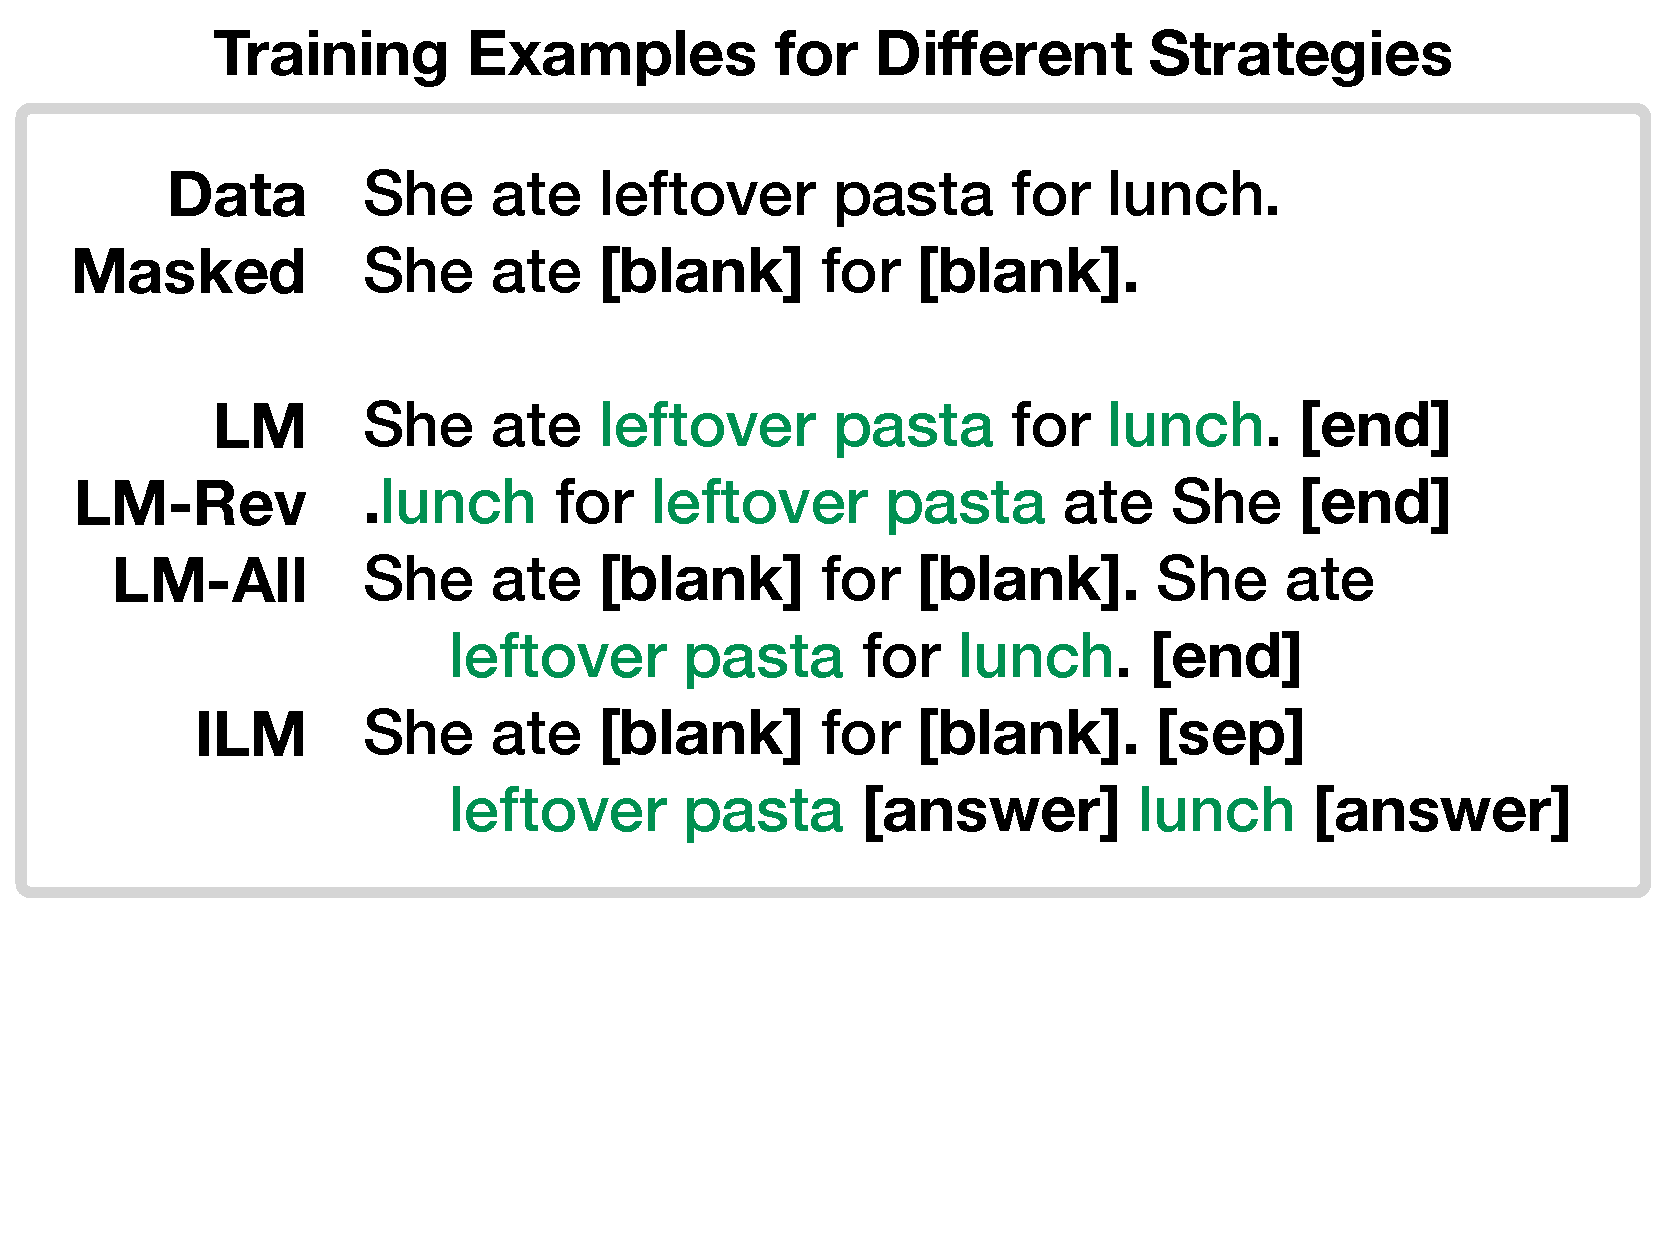
\includegraphics[width=1\linewidth]{acl2020-templates/figures/ilm_figure2_final.pdf}
    \vspace{-2cm}
    \caption{
    Training examples for three baseline infilling strategies and ILM on a given artificially-masked sentence. 
    For each strategy, we train the same architecture (GPT-2) on such examples. 
    At both training and test time, examples are fed from left to right; anything to the left of a green target is available to the model as context when predicting the target.
    Precisely, \lm{} only considers past context, and \lmrev{} only considers future. \lmall{} considers all available context but uses long sequence lengths. Our proposed \ilm{} considers all context while using fewer tokens. 
    %For all strategies, we compute model performance \emph{only} on the masked (green) tokens (here, the tokens ``leftover,'' ``pasta,'' and ``lunch'').
    }
    \label{fig:training_examples}
\end{figure}

For all experiments, we train the same architecture (GPT-2 ``small'') using the same hyperparameters (\Cref{sec:hyperparams}) while varying the infilling strategy and dataset. 
In addition to our proposed \ilm{} strategy for infilling, we consider three baseline strategies:
(1)~language modeling (\lm{}; ``infilling'' based only on past context),
(2)~reverse language modeling (\lmrev{}; ``infilling'' based only on future context),
and 
(3)~language modeling based on all available context (\lmall{}).
\lmall{} simply concatenates $\x$ and $\xtilde$ together as in~\citet{fedus2018maskgan}. 
\lmall{} represents arguably the simplest way one could conceive of infilling with LMs, 
but results in long sequence lengths.
Training examples for all strategies are depicted in \Cref{fig:training_examples}.

For each strategy, we also vary whether training is initialized from the pre-trained GPT-2 model or from scratch.
Despite discrepancies between the pre-training and our fine-tuning for most infilling strategies, 
\emph{all} of the infilling experiments initialized from the pre-trained checkpoint performed better than their from-scratch counterparts.
This indicates that ILM can effectively leverage large-scale language modeling pre-training to improve infilling performance. 
Henceforth, we will only discuss the models initialized from the pre-trained checkpoint, though we report quantitative performance for all models in \Cref{sec:eval_granularities}.

For the models trained on \stories{} and \abstracts{}, we trained models to convergence using early stopping based on the validation set perplexity (PPL) of each model computed only on the masked tokens. 
These models took about a day to reach their early stopping criteria on a single GPU. 
For the larger \lyrics{} dataset, we trained models for $2$ epochs (about two days on a single GPU). 